\documentclass[12pt,pdflatex]{elsarticle} 
% this is edited by MDW to try to get to the 10000 word limit
% November 2, 2016
%%%%%%%%%%%%%%%%%%%%%%%%%%%%%%%%%%%%%%%%%%%%%%%%%%
%%%%%%%%%%%%%%%%%%%% PREAMBLE %%%%%%%%%%%%%%%%%%%%
%%%%%%%%%%%%%%%%%%%%%%%%%%%%%%%%%%%%%%%%%%%%%%%%%%


% -------------------- defaults -------------------- %
% load lots o' packages

% references
\usepackage{natbib}

% Fonts
\usepackage[default,osfigures,scale=0.95]{opensans}
\usepackage[T1]{fontenc}
\usepackage{ae}
% to colorize links in document. See color specification below
\usepackage[pdftex,hyperref,x11names]{xcolor}
% load the hyper-references package and set document info
\usepackage[pdftex]{hyperref}

% Generate some fake text
\usepackage{blindtext}

% layout control
\usepackage{geometry}
\geometry{verbose,tmargin=1.25in,bmargin=1.25in,lmargin=1.1in,rmargin=1.1in}
\usepackage{parallel}
\usepackage{parcolumns}
\usepackage{fancyhdr}

% math typesetting
\usepackage{array}
\usepackage{amsmath}
\usepackage{amssymb}
\usepackage{amsfonts}
\usepackage{relsize}
\usepackage{mathtools}
\usepackage{bm}
\usepackage[%
decimalsymbol=.,
digitsep=fullstop
]{siunitx}

% restricts float objects to be inserted before end of section
% creates float barriers
\usepackage[section]{placeins}

% tables
\usepackage{tabularx}
\usepackage{booktabs}
\usepackage{multicol}
\usepackage{multirow}
\usepackage{longtable}

% to adapt caption style
\usepackage[font={small},labelfont=bf]{caption}

% footnotes at bottom
\usepackage[bottom]{footmisc}
   \renewcommand{\footnotelayout}{\doublespacing} % set spacing in footnotes
   \newlength{\myfootnotesep}
   \setlength{\myfootnotesep}{\baselineskip}
   \addtolength{\myfootnotesep}{-\footnotesep}
   \setlength{\footnotesep}{\myfootnotesep} % set spacing between footnotes

% to change enumeration symbols begin{enumerate}[(a)]
\usepackage{enumerate}

% to make enumerations and itemizations within paragraphs or
% lines. f.i. begin{inparaenum} for (a) is (b) and (c)
\usepackage{paralist}

% graphics stuff
\usepackage{subfig}
\usepackage{graphicx}
\usepackage[space]{grffile} % allows us to specify directories that have spaces
\usepackage{placeins} % prevents floats from moving past a \FloatBarrier
\usepackage{tikz}
\usepackage{rotating}

% Spacing
\usepackage[doublespacing]{setspace}

% -------------------------------------------------- %


% -------------------- page template -------------------- %

\setlength{\headheight}{15pt}
\setlength{\headsep}{20pt}
\pagestyle{fancyplain}
 
\fancyhf{}
 
\lhead{\fancyplain{}{}}
\chead{\fancyplain{}{Amen for LFM}}
\rhead{\fancyplain{}{\today}}
\rfoot{\fancyplain{}{\thepage}}

% ----------------------------------------------- %


% -------------------- customizations -------------------- %

% easy commands for number propers
\newcommand{\first}{$1^{\text{st}}$}
\newcommand{\second}{$2^{\text{nd}}$}
\newcommand{\third}{$3^{\text{rd}}$}
\newcommand{\nth}[1]{${#1}^{\text{th}}$}

% easy command for boldface math symbols
\newcommand{\mbs}[1]{\boldsymbol{#1}}

% command for R package font
\newcommand{\pkg}[1]{{\fontseries{b}\selectfont #1}}

% approx iid
\newcommand\simiid{\stackrel{\mathclap{\normalfont\mbox{\tiny{iid}}}}{\sim}}

% -------------------------------------------------------- %

%%%%%%%%%%%%%%%%%%%%%%%%%%%%%%%%%%%%%%%%%%%%%%%%%%
%%%%%%%%%%%%%%%%%%%% DOCUMENT %%%%%%%%%%%%%%%%%%%%
%%%%%%%%%%%%%%%%%%%%%%%%%%%%%%%%%%%%%%%%%%%%%%%%%%

% remove silly elsevier preprint note
\makeatletter
\def\ps@pprintTitle{%
 \let\@oddhead\@empty
 \let\@evenhead\@empty
 \def\@oddfoot{}%
 \let\@evenfoot\@oddfoot}

% \def\input@path{{/Users/janus829/Dropbox/Research/netModels/summResults/}, {/Users/s7m/Dropbox/Research/netModels/summResults/}, {/Users/mdw/Dropbox/netModels/summResults/}}
% \graphicspath{{/Users/janus829/Dropbox/Research/netModels/summResults/}, {/Users/s7m/Dropbox/Research/netModels/summResults/},{/Users/mdw/Dropbox/netModels/summResults/}}
\makeatother

\begin{document}

% saying hello ----------------------------------------------- %
\thispagestyle{empty}
\begin{frontmatter}

\title{Supporting Information for ``Inferential Approaches for Network Analysis: AMEN for Latent Factor Models''}\tnoteref{t1}

\tnotetext[t1]{S.M. and M.W. acknowledge support from National Science Foundation (NSF) Award 1259266 and P.H. acknowledges support from NSF Award 1505136.}

\author[msu]{Shahryar Minhas\corref{cor1}}
\ead{s7.minhas@gmail.com}
\cortext[cor1]{Corresponding author}
\author[duke2]{Peter D. Hoff}
\author[duke]{Michael D. Ward}

\address[msu]{Department of Political Science, Michigan State University, East Lansing, MI 48824, USA}
\address[duke]{Department of Political Science, Duke University, Durham, NC 27701, USA}
\address[duke2]{Department of Statistical Science, Duke University, Durham, NC 27701, USA}

% \begin{abstract}
% There is growing interest in the study of social networks enabling  scholars to move away from focusing on individual observations to examining more precisely the interrelationships among observations. Many network approaches have been developed in a descriptive fashion, but attention to inferential approaches using statistical models of networks has been growing. We review a latent factor approach that models interdependencies among observations using additive and multiplicative effects (AME) which can be applied to binary, ordinal, and continuous network data. We compare  this to alternative latent variable models as well as to exponential random graph models (ERGM). The AME approach can be easily implemented in the context of general linear models. It is both computationally straightforward and avoids degeneracy, which often plagues ERGM. In an out-of-sample context, it out-performs alternatives in terms of predicting links and capturing network dependencies.
% \end{abstract}

\end{frontmatter}
% ----------------------------------------------- %

\newpage\setcounter{page}{1}

\section*{Additive and Multiplicative Effects Gibbs Sampler}

To estimate, the effects of our exogenous variables and latent attributes we utilize a Bayesian probit model in which we sample from the posterior distribution of the full conditionals until convergence. Specifically, given observed data $\textbf{Y}$ and $\textbf{X}$ -- where $\textbf{X}$ is a design array that includes our sender, receiver, and dyadic covariates -- we estimate our network of binary ties using a probit framework where: $y_{ij,t} = 1(\theta_{ij,t}>0)$ and $\theta_{ij,t} = \bm\beta^{\top}\mathbf{X}_{ij,t} + a_{i} + b_{j} + \textbf{u}_{i}^{\top} \textbf{D} \textbf{v}_{j} + \epsilon_{ij}$. The derivation of the full conditionals is described in detail in \citet{hoff:2005} and \citet{hoff:2008}, thus here we only outline the Markov chain Monte Carlo (MCMC) algorithm for the AME model that we utilize in this paper.

\begin{itemize}
 \item Given initial values of $\{\bm\beta, \textbf{a}, \textbf{b}, \textbf{U}, \textbf{V}, \Sigma_{ab}, \rho, \text{ and } \sigma_{\epsilon}^{2}\}$, the algorithm proceeds as follows:
 \begin{itemize}
 	\item sample $\bm\theta \; | \;  \bm\beta, \textbf{X}, \bm\theta, \textbf{a}, \textbf{b}, \textbf{U}, \textbf{V}, \Sigma_{ab}, \rho, \text{ and } \sigma_{\epsilon}^{2}$ (Normal)
 	\item sample $\bm\beta \; | \;  \textbf{X}, \bm\theta, \textbf{a}, \textbf{b}, \textbf{U}, \textbf{V}, \Sigma_{ab}, \rho, \text{ and } \sigma_{\epsilon}^{2}$ (Normal)
 	\item sample $\textbf{a}, \textbf{b} \; | \; \bm\beta, \textbf{X}, \bm\theta, \textbf{U}, \textbf{V}, \Sigma_{ab}, \rho, \text{ and } \sigma_{\epsilon}^{2}$ (Normal)
	\item sample $\Sigma_{ab} \; | \; \bm\beta, \textbf{X}, \bm\theta, \textbf{a}, \textbf{b}, \textbf{U}, \textbf{V}, \rho, \text{ and } \sigma_{\epsilon}^{2}$ (Inverse-Wishart)
 	\item update $\rho$ using a Metropolis-Hastings step with proposal $p^{*} | p  \sim$ truncated normal$_{[-1,1]}(\rho, \sigma_{\epsilon}^{2})$
 	\item sample $\sigma_{\epsilon}^{2} \; | \; \bm\beta, \textbf{X}, \bm\theta, \textbf{a}, \textbf{b}, \textbf{U}, \textbf{V}, \Sigma_{ab}, \text{ and } \rho$ (Inverse-Gamma)
 	\item For each $k \in K$:
 	\begin{itemize}
 		\item Sample $\textbf{U}_{[,k]} \; | \; \bm\beta, \textbf{X}, \bm\theta, \textbf{a}, \textbf{b}, \textbf{U}_{[,-k]}, \textbf{V}, \Sigma_{ab}, \rho, \text{ and } \sigma_{\epsilon}^{2}$ (Normal)
 		\item Sample $\textbf{V}_{[,k]} \; | \; \bm\beta, \textbf{X}, \bm\theta, \textbf{a}, \textbf{b}, \textbf{U}, \textbf{V}_{[,-k]}, \Sigma_{ab}, \rho, \text{ and } \sigma_{\epsilon}^{2}$ (Normal)
 		\item Sample $\textbf{D}_{[k,k]}  \; | \; \bm\beta, \textbf{X}, \bm\theta, \textbf{a}, \textbf{b}, \textbf{U}, \textbf{V}, \Sigma_{ab}, \rho, \text{ and } \sigma_{\epsilon}^{2}$ (Normal)\footnote{Subsequent to estimation, \textbf{D} matrix is absorbed into the calculation for $\textbf{V}$ as we iterate through $K$. }
 	\end{itemize}
 \end{itemize}
\end{itemize}

\clearpage
\section*{Ingold \& Fischer Model Specification and Expected Effects}

\newcolumntype{L}{>{\arraybackslash}m{9cm}}
\begin{table}[ht]
\centering
\begingroup\scriptsize
\begin{tabular}{lLc}
\footnotesize{\textbf{Variable}} & \footnotesize{\textbf{Description}} & \footnotesize{\textbf{Expected Effect}} \\ \hline\hline
	\multicolumn{3}{l}{\textbf{Conflicting policy preferences}} \\
	\quad Business v. NGO & Binary, dyadic covariate that equals one when one actor is from the business sector and the other an NGO. & $-$ \\
	\quad Opposition/alliance & Binary, dyadic covariate that equals one when $i$, sender, perceives $j$, receiver, as having similar policy objectives regarding climate change.  & $+$ \\
	\quad Preference dissimilarity & Transformation of four core beliefs into a Manhattan distance matrix, smaller the distance the closer the beliefs of $i$ and $j$. & $-$ \\
	\multicolumn{3}{l}{\textbf{Transaction costs}} \\
	\quad Joint forum participation & Binary, dyadic covariate that equals one when $i$ and $j$ belong to the same policy forum. & $+$ \\
	\multicolumn{3}{l}{\textbf{Influence}} \\
	\quad Influence attribution & Binary, dyadic covariate that equals one when $i$ considers $j$ to be influential. & $+$ \\
	\quad Alter's influence in-degree & Number of actors that mention $i$ as being influential, this is a measure of reputational power. & $+$ \\
	\quad Influence absolute diff. & Absolute difference in reputational power between $i$ and $j$. & $-$ \\
	\quad Alter = Government Actor & Binary, nodal covariate that equals one when $j$ is a state actor. & $+$ \\
	\multicolumn{3}{l}{\textbf{Functional requirements}} \\
	\quad Ego = Environment NGO & Binary, nodal covariate that equals one when $i$ is an NGO. & $+$ \\
	\quad Same actor type & Binary, dyadic covariate that equals when $i$ and $j$ are the same actor type. & $+$ \\
	\multicolumn{3}{l}{\textbf{Endogenous dependencies: ERGM Specific Parameters}} \\
	\quad Mutuality & Captures concept of reciprocity, if $i$ indicates they collaborated with $j$ then $j$ likely collaborates with $i$. & $+$\\
	\quad Outdegree popularity & Captures idea that actors sending more ties will be more popular targets themselves for collaboration.  & $+$ \\
	\quad Twopaths & Counts the number of two-paths in the network, two-path is an instance where $i$ is connected to $j$, $j$ to $k$, but $i$ is not connected to $k$. & $-$ \\
	\quad GWIdegree (2.0) & Takes into account how many ties a node sends in the network, used to capture network structures that result from some highly active nodes.  & $+$ \\
	\quad GWESP (1.0) & Counts the number of shared partners for each pair and sums across.  & $+$ \\
	\quad GWOdegree (0.5) & Takes into account how many ties a node receives in the network, used to capture networks structures that result from some highly popular nodes.  & $+$ \\
\hline\hline
\end{tabular}
\endgroup
\caption{Summary of variables to be included in model specification.}
\label{tab:theorySpec}
\end{table}
\FloatBarrier

\clearpage
\subsection*{AME Model Convergence}
\label{sec:ameConvAppendix}

Trace plot for AME model presented in paper.

\begin{figure}[ht]
	\centering
	\begin{tabular}{cc}
	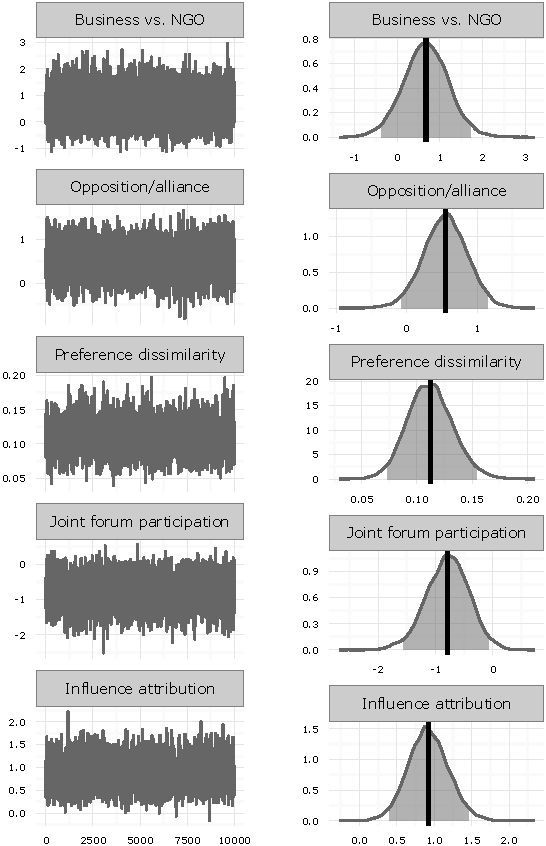
\includegraphics[width=.45\textwidth]{ameConv1_SR2} &
	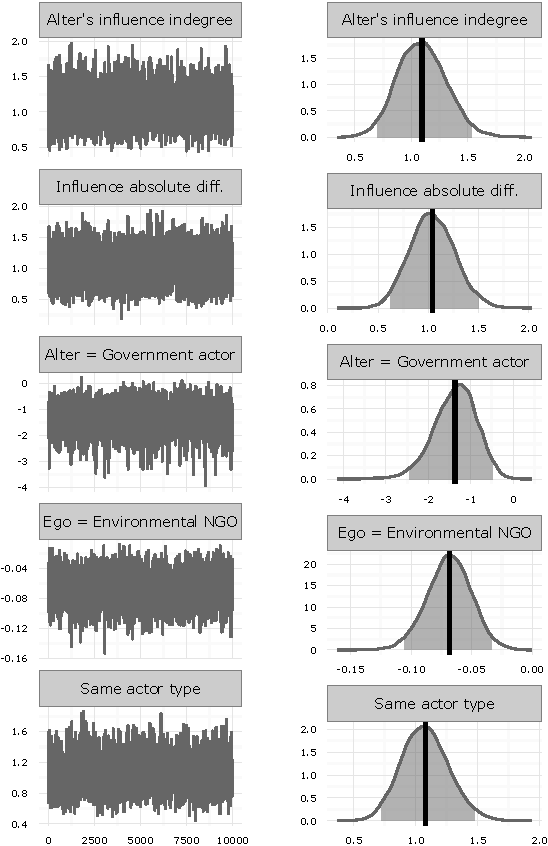
\includegraphics[width=.45\textwidth]{ameConv2_SR2}
	\end{tabular}
	\caption{Trace plot for AME model presented in paper. In this model, we utilize the SRM to account for first and second-order dependence. To account for third order dependencies we use the latent factor approach with $K=2$.}
	\label{fig:ameConv}
\end{figure}
\FloatBarrier
\newpage

\section*{Multiplicative Effects Visualization}

When it comes to estimating higher-order effects, ERGM is able to provide explicit estimates of a variety of higher-order parameters, however, this comes with the caveat that these are the ``right'' set of endogenous dependencies. The AME approach, as shown in Equation~\ref{eqn:ame}, estimates network dependencies by examining patterns left over after taking into account the observed covariates. For the sake of space, we focus on examining the third-order dependencies left over after accounting for the observed covariates and network covariance structure modeled by the SRM. A visualization of remaining third-order dependencies is shown in Figure~\ref{fig:uv}.

\begin{figure}[ht]
\centering
	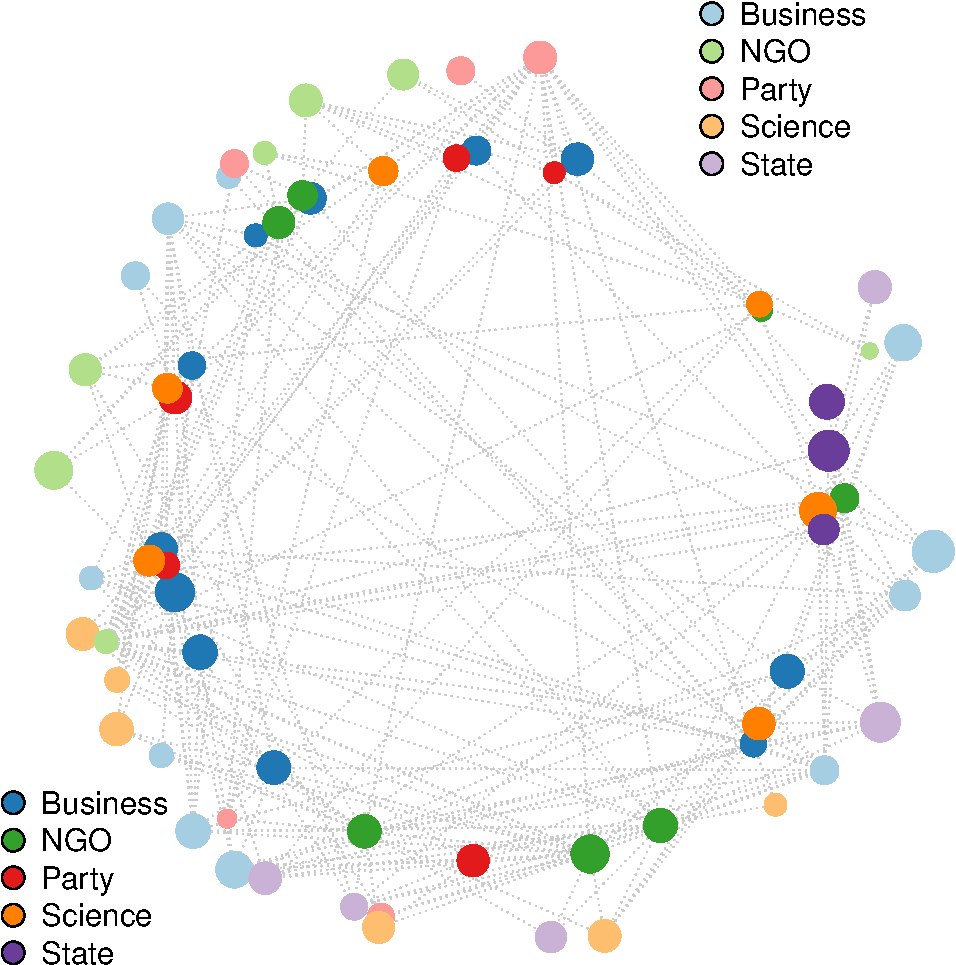
\includegraphics[width=.5\textwidth]{ameFitSR_2_UV}
	\caption{Circle plot of estimated latent factors.}
	\label{fig:uv}
\end{figure}
\FloatBarrier

In Figure~\ref{fig:uv}, the directions of $\hat{u}_{i}$'s and $\hat{v}_{i}$'s are noted in lighter and darker shades, respectively, of an actor's type.\footnote{For example, actors from industry and business are assigned a color of blue and the direction of $\hat{u}_{i}$ for these actors is shown in light blue and $\hat{v}_{i}$ in dark blue} The size of actors is a function of the magnitude of the vectors, and dashed lines between actors indicate greater than expected levels of collaboration based on the regression term and additive effects. In the case of the application dataset that we are using here organization names have been anonymized and no additional covariate information is available. However, if we were to observe nodes sharing certain attributes clustering together in this circle plot that would mean such an attribute could be an important factor in helping us to understand collaborations among actors in this network. Given how actors of different types are distributed in almost a random fashion in this plot, we can at least be sure that it is unlikely other third-order patterns can be picked up by that factor.

\clearpage
\section*{Other Network Goodness of Fit Tests}
\label{sec:otherNetGof}

Below we show a standard set of statistics upon which comparisons are usually conducted:\footnote{See \citet{morris:etal:2008} for details on each of these parameters. If one was to examine goodness of fit in the \pkg{ergm} package these parameters would be calculated by default.}

\newcolumntype{L}{>{\arraybackslash}m{9cm}}
\begin{table}[ht]
\centering
\begingroup\scriptsize
\begin{tabular}{lL}
\footnotesize{\textbf{Variable}} & \footnotesize{\textbf{Description}} \\ \hline\hline
	Dyad-wise shared partners & Number of dyads in the network with exactly $i$ shared partners. \\
	Edge-wise shared partners & Similar to above except this counts the number of dyads with the same number of edges. \\
	Geodesic distances & The proportion of pairs of nodes whose shortest connecting path is of length $k$, for $k=1,2,\ldots$. Also, pairs of nodes that are not connected are classified as $k=\infty$. \\
	Incoming k-star & Propensities for individuals to have connections with multiple network partners. \\
	Indegree & Proportion of nodes with the same value of the attribute as the receiving node. \\
	Outdegree & Proportion of nodes with the same value of the attribute as the sending node. \\
\hline\hline
\end{tabular}
\endgroup
\caption{Description of a set of standard statistics used to assess whether a model captures network dependencies. }
\label{tab:netStat}
\end{table}
\FloatBarrier

We simulate 1,000 networks from the LSM, ERGM, and AME model and compare how well they align with the observed network in terms of the statistics described in Table~\ref{tab:netStat}. The results are shown in Figure~\ref{fig:gofAll}. Values for the observed network are indicated by a gray bar and average values from the simulated networks for the AME, ERGM, and LSM are represented by a diamond, triangle, and square, respectively. The densely shaded interval around each point represents the 95\% interval from the simulations and the taller, less dense the 90\% interval.\footnote{Calculation for the incoming k-star statistic is not currently supported by the \pkg{latentnet} package.} Looking across the panels in Figure~\ref{fig:gofAll} it is clear that there is little difference between the ERGM and AME models in terms of how well they capture network dependencies. The LSM model, however, does perform somewhat worse in comparison here as well. Particularly, when it comes to assessing the number of edge-wise shared partners and in terms of capturing the indegree and outdegree distributions of the collaboration network.

\begin{figure}[ht]
	\centering
	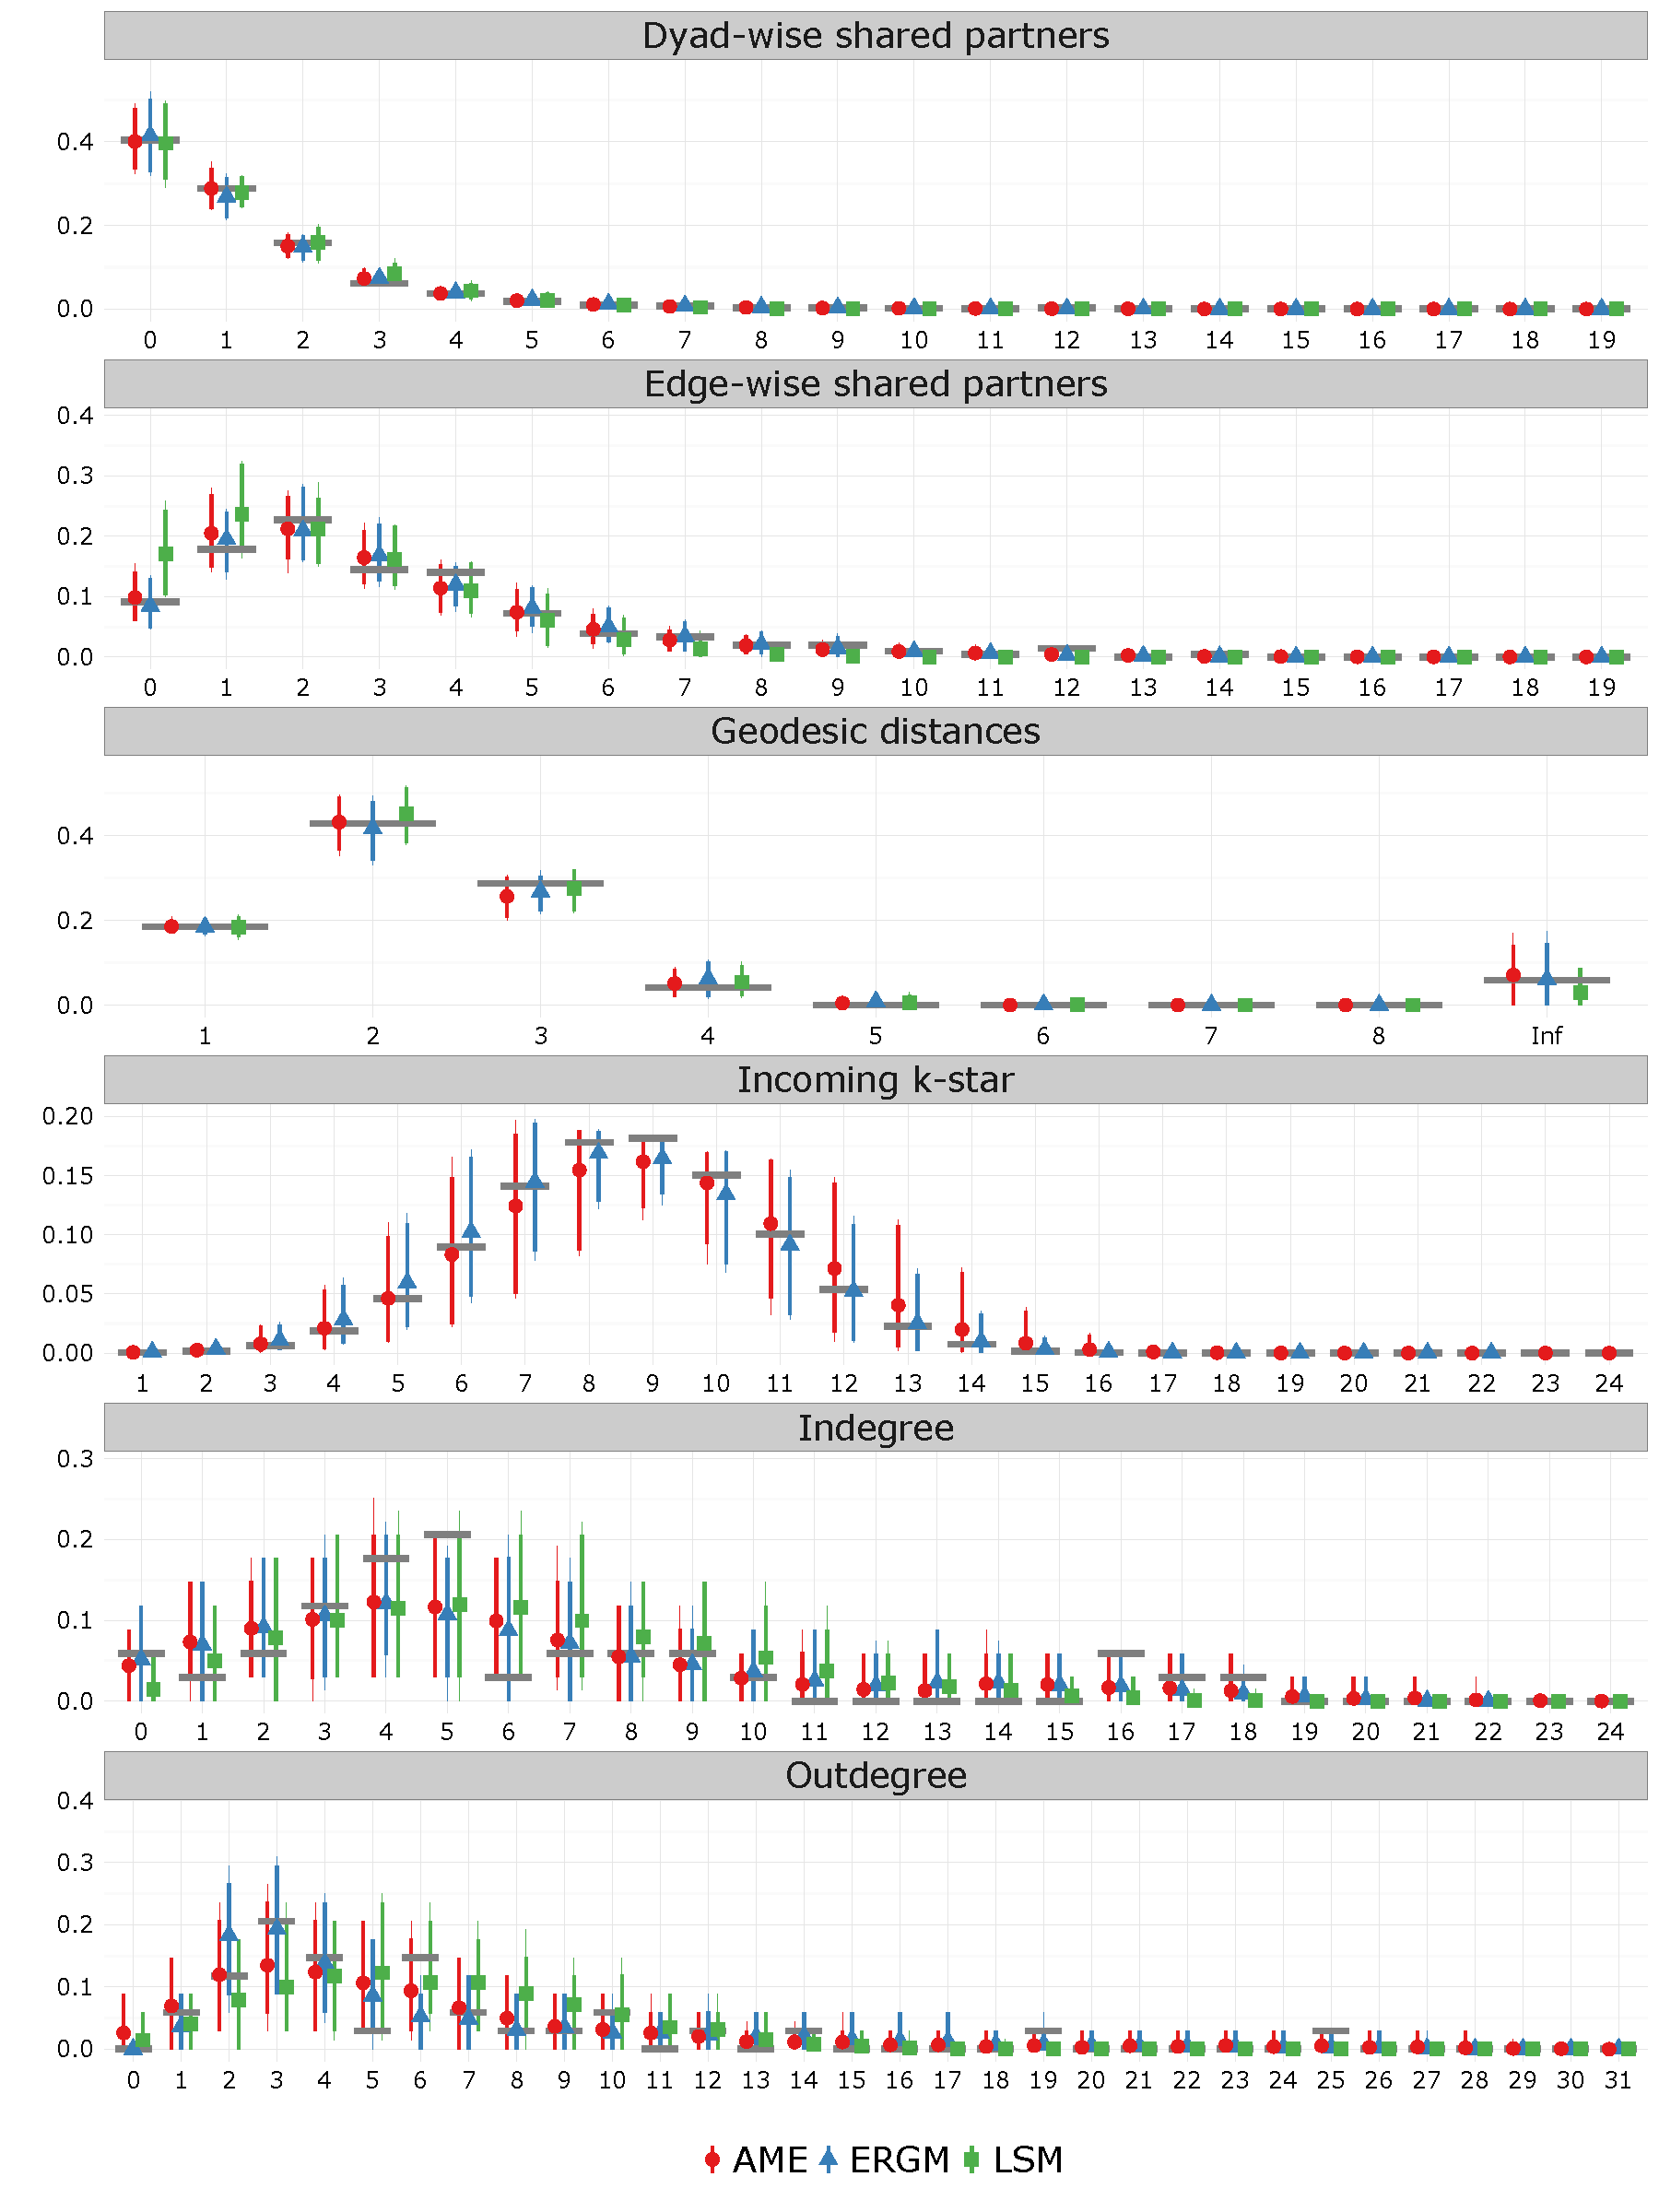
\includegraphics[width=1\textwidth]{ggGofAll}
	\caption{Goodness of fit statistics to assess how well the LSM, ERGM, and AME approaches account for network dependencies.}
	\label{fig:gofAll}
\end{figure}
\FloatBarrier

\clearpage
\section*{Comparison of \pkg{amen} \& \pkg{latentnet} $\sf{R}$ Packages}
\label{sec:ameVsLatentnetAppendix}

Here we provide a comparison of the AME model we present in the paper with a variety of parameterizations from the \pkg{latentnet} package. The number of dimensions in the latent space in each of these cases is set to 2. LSM (SR) represents a model in which random sender and receiver effects are included. 

% latex table generated in R 3.4.0 by xtable 1.8-2 package
% Thu Jun 22 00:28:27 2017
\begin{table}[ht]
\centering
\begingroup\footnotesize
\begin{tabular}{lccc}
   & LSM & LSM (SR) & AME \\ 
  \hline
\hline
Intercept/Edges & 0.94 & 0.60 & -3.39 \\ 
   & [0.09; 1.82] & [-1.10; 2.37] & [-4.38; -2.50] \\ 
  \textbf{Conflicting policy preferences} &  &  &  \\ 
  $\;\;\;\;$ Business vs. NGO & -1.37 & -3.07 & -1.37 \\ 
   & [-2.42; -0.41] & [-4.77; -1.56] & [-2.44; -0.47] \\ 
  $\;\;\;\;$ Opposition/alliance & 0.00 & 0.31 & 1.08 \\ 
   & [-0.40; 0.39] & [-0.24; 0.86] & [0.72; 1.47] \\ 
  $\;\;\;\;$ Preference dissimilarity & -1.76 & -1.88 & -0.79 \\ 
   & [-2.62; -0.90] & [-3.07; -0.68] & [-1.55; -0.08] \\ 
  \textbf{Transaction costs} &  &  &  \\ 
  $\;\;\;\;$ Joint forum participation & 1.51 & 1.56 & 0.92 \\ 
   & [0.86; 2.17] & [0.69; 2.41] & [0.40; 1.47] \\ 
  \textbf{Influence} &  &  &  \\ 
  $\;\;\;\;$ Influence attribution & 0.08 & 0.30 & 1.09 \\ 
   & [-0.40; 0.55] & [-0.37; 0.96] & [0.69; 1.53] \\ 
  $\;\;\;\;$ Alter's influence indegree & 0.01 & 0.06 & 0.11 \\ 
   & [-0.03; 0.04] & [-0.03; 0.14] & [0.07; 0.15] \\ 
  $\;\;\;\;$ Influence absolute diff. & 0.04 & -0.08 & -0.07 \\ 
   & [-0.01; 0.09] & [-0.14; -0.02] & [-0.11; -0.03] \\ 
  $\;\;\;\;$ Alter = Government actor & -0.46 & -0.11 & 0.55 \\ 
   & [-1.08; 0.14] & [-1.91; 1.76] & [-0.07; 1.15] \\ 
  \textbf{Functional requirements} &  &  &  \\ 
  $\;\;\;\;$ Ego = Environmental NGO & -0.60 & -1.69 & 0.67 \\ 
   & [-1.32; 0.09] & [-3.74; 0.23] & [-0.38; 1.71] \\ 
  $\;\;\;\;$ Same actor type & 1.17 & 1.82 & 1.04 \\ 
   & [0.63; 1.71] & [1.10; 2.54] & [0.63; 1.50] \\ 
   \hline
\hline
\end{tabular}
\endgroup
\caption{95\% posterior credible intervals are provided in brackets.}
\label{tab:regTable_latSpace}
\end{table}



\begin{figure}[ht]
	\centering
	\begin{tabular}{cc}
	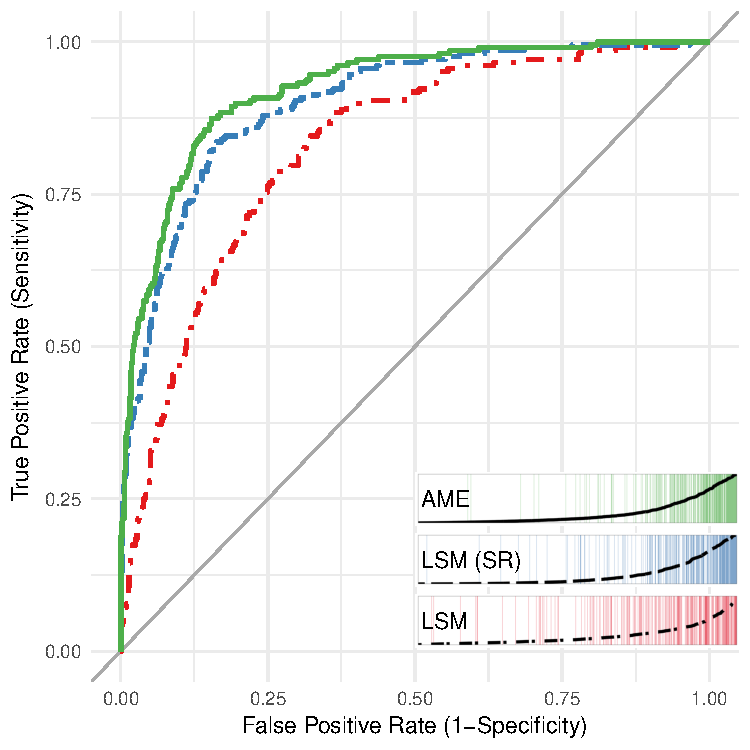
\includegraphics[width=.5\textwidth]{roc_latSpace_outSampleSmall} &
	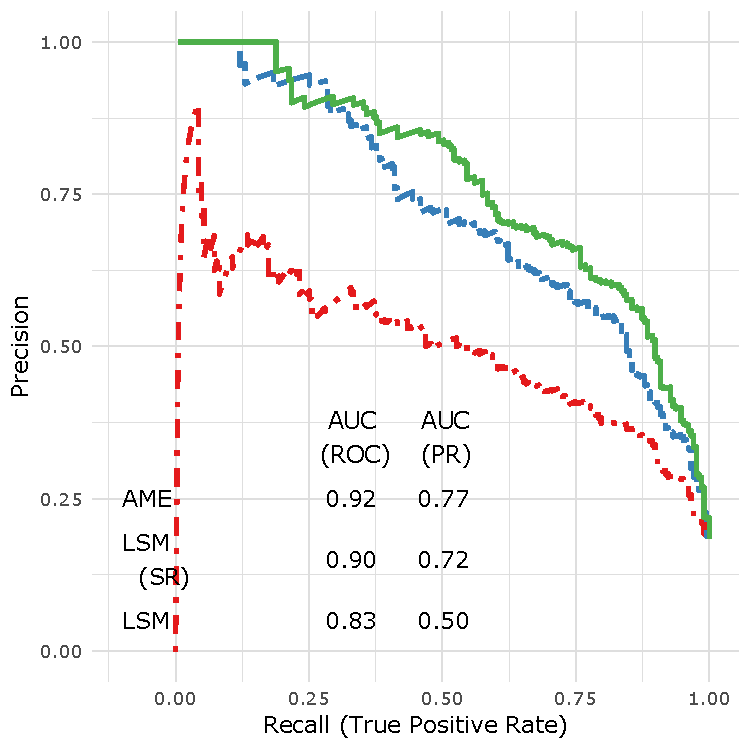
\includegraphics[width=.5\textwidth]{rocPr_latSpace_outSampleSmall}
	\end{tabular}
	\caption{Assessments of out-of-sample predictive performance using ROC curves, separation plots, and PR curves. AUC statistics are provided as well for both curves.}
	\label{fig:roc_latentSpace}
\end{figure}

\begin{figure}[ht]
	\centering
	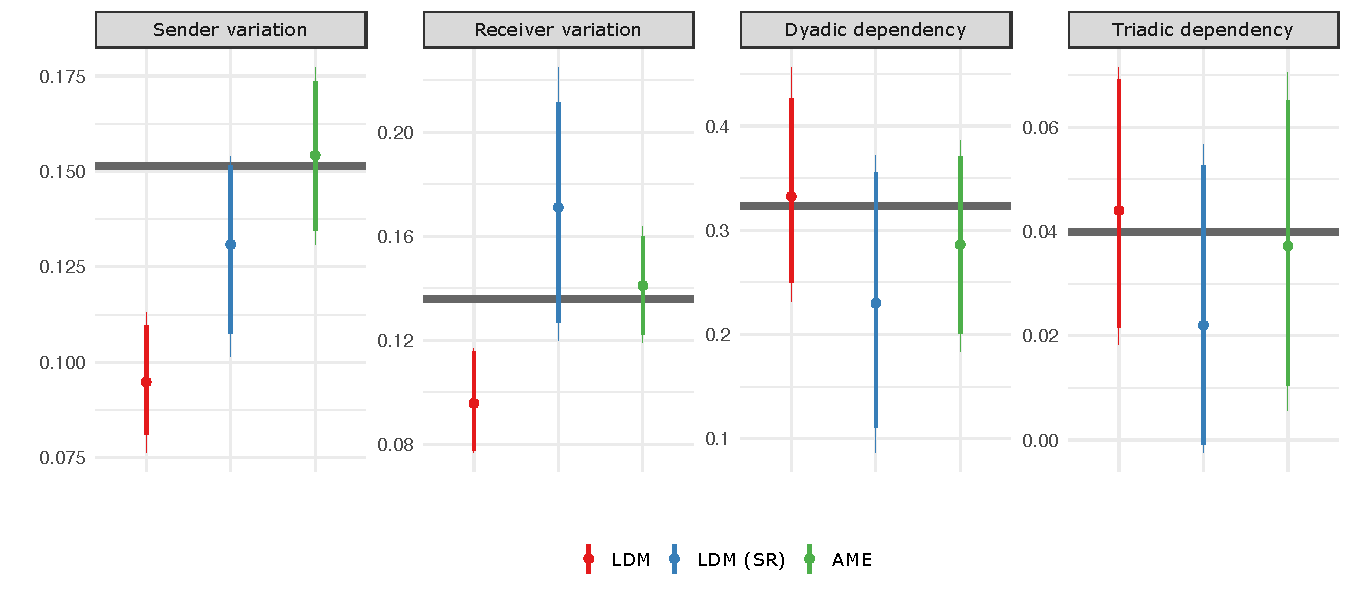
\includegraphics[width=1\textwidth]{netPerfCoef_latSpaceSmall}
	\caption{Network goodness of fit summary using \pkg{amen}.}
	\label{fig:netPerfCoef_latSpace}
\end{figure}

\FloatBarrier

\clearpage
\section*{Comparison with other AME Parameterizations}
\label{sec:ameVsAmeAppendix}

Here we provide a comparison of the AME model we present in the paper that uses $K=2$ for multiplicative effects and show how results change when we use $K=\{1,3,4\}$. Trace plots for $K=\{1,3,4\}$ are available upon request.

% latex table generated in R 3.3.1 by xtable 1.8-2 package
% Tue Sep 27 12:34:36 2016
\begin{table}[ht]
\centering
\begingroup\footnotesize
\begin{tabular}{lcccc}
   & AME (k=1) & AME (k=2) & AME (k=3) & AME (k=4) \\
  \hline
\hline
Intercept/Edges & -3.08 & -3.39 & -3.72 & -3.93 \\
   & [-3.91; -2.30] & [-4.38; -2.50] & [-4.84; -2.73] & [-5.12; -2.87] \\
  \textbf{Conflicting policy preferences} &  &  &  &  \\
  $\;\;\;\;$ Business vs. NGO & -1.28 & -1.37 & -1.48 & -1.51 \\
   & [-2.20; -0.47] & [-2.44; -0.47] & [-2.63; -0.49] & [-2.69; -0.47] \\
  $\;\;\;\;$ Opposition/alliance & 0.95 & 1.08 & 1.19 & 1.28 \\
   & [0.64; 1.27] & [0.72; 1.47] & [0.80; 1.64] & [0.86; 1.77] \\
  $\;\;\;\;$ Preference dissimilarity & -0.65 & -0.79 & -0.89 & -0.95 \\
   & [-1.30; -0.03] & [-1.55; -0.08] & [-1.71; -0.12] & [-1.80; -0.14] \\
  \textbf{Transaction costs} &  &  &  &  \\
  $\;\;\;\;$ Joint forum participation & 0.84 & 0.92 & 1.01 & 1.06 \\
   & [0.38; 1.31] & [0.40; 1.47] & [0.44; 1.62] & [0.43; 1.72] \\
  \textbf{Influence} &  &  &  &  \\
  $\;\;\;\;$ Influence attribution & 1.00 & 1.09 & 1.21 & 1.28 \\
   & [0.63; 1.39] & [0.69; 1.53] & [0.75; 1.71] & [0.80; 1.84] \\
  $\;\;\;\;$ Alter's influence indegree & 0.10 & 0.11 & 0.12 & 0.13 \\
   & [0.07; 0.14] & [0.07; 0.15] & [0.08; 0.17] & [0.09; 0.18] \\
  $\;\;\;\;$ Influence absolute diff. & -0.06 & -0.07 & -0.07 & -0.08 \\
   & [-0.10; -0.03] & [-0.11; -0.03] & [-0.12; -0.04] & [-0.12; -0.04] \\
  $\;\;\;\;$ Alter = Government actor & 0.52 & 0.55 & 0.60 & 0.64 \\
   & [-0.04; 1.07] & [-0.07; 1.15] & [-0.07; 1.27] & [-0.07; 1.35] \\
  \textbf{Functional requirements} &  &  &  &  \\
  $\;\;\;\;$ Ego = Environmental NGO & 0.61 & 0.67 & 0.76 & 0.80 \\
   & [-0.31; 1.56] & [-0.38; 1.71] & [-0.38; 1.90] & [-0.40; 2.04] \\
  $\;\;\;\;$ Same actor type & 0.97 & 1.04 & 1.11 & 1.17 \\
   & [0.60; 1.35] & [0.63; 1.50] & [0.64; 1.59] & [0.68; 1.68] \\
   \hline
\hline
\end{tabular}
\endgroup
\caption{95\% posterior credible intervals are provided in brackets.}
\label{tab:regTable_ame}
\end{table}


\begin{figure}[ht]
	\centering
	\begin{tabular}{cc}
	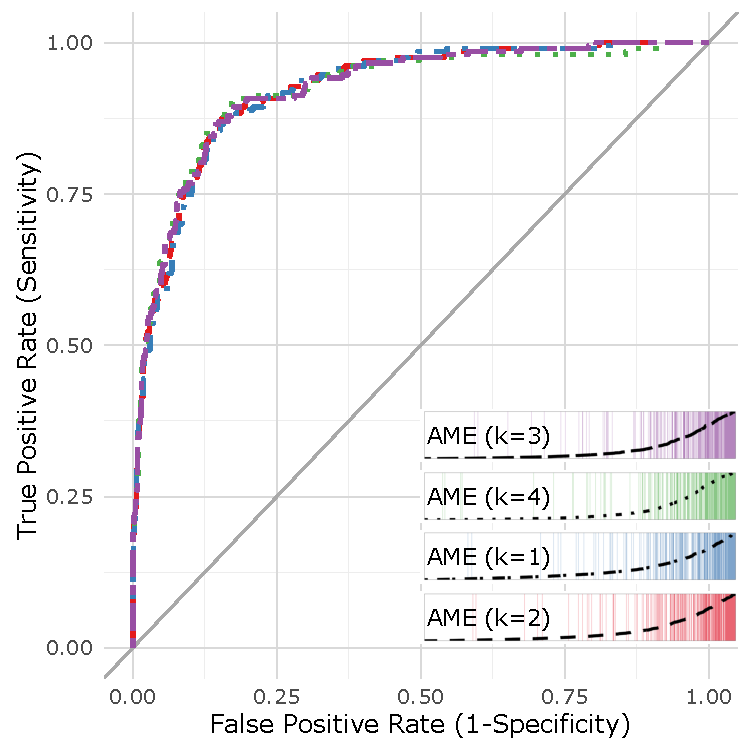
\includegraphics[width=.5\textwidth]{roc_ameSR_outSample} &
	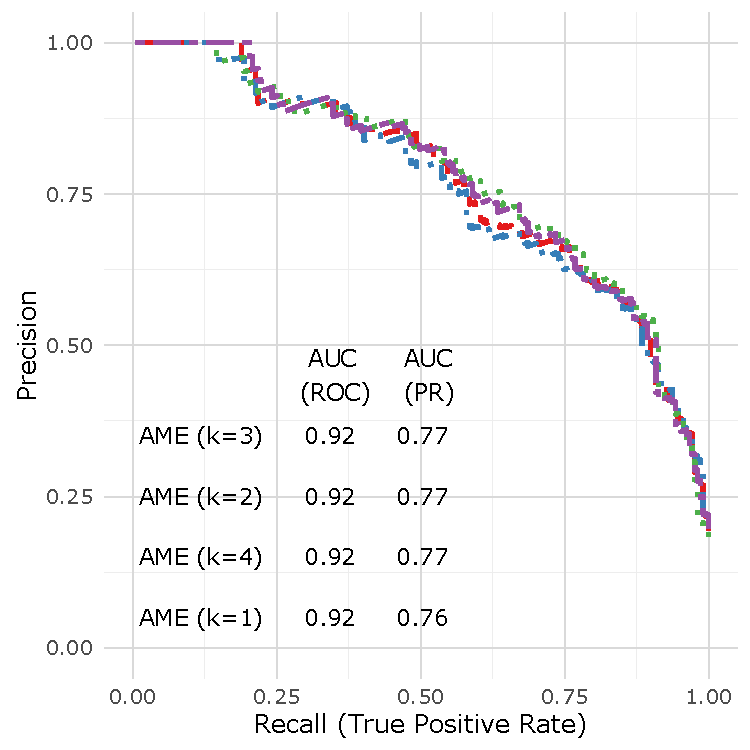
\includegraphics[width=.5\textwidth]{rocPr_ameSR_outSample}
	\end{tabular}
	\caption{Assessments of out-of-sample predictive performance using ROC curves, separation plots, and PR curves. AUC statistics are provided as well for both curves.}
	\label{fig:roc_ame}
\end{figure}

\begin{figure}[ht]
	\centering
	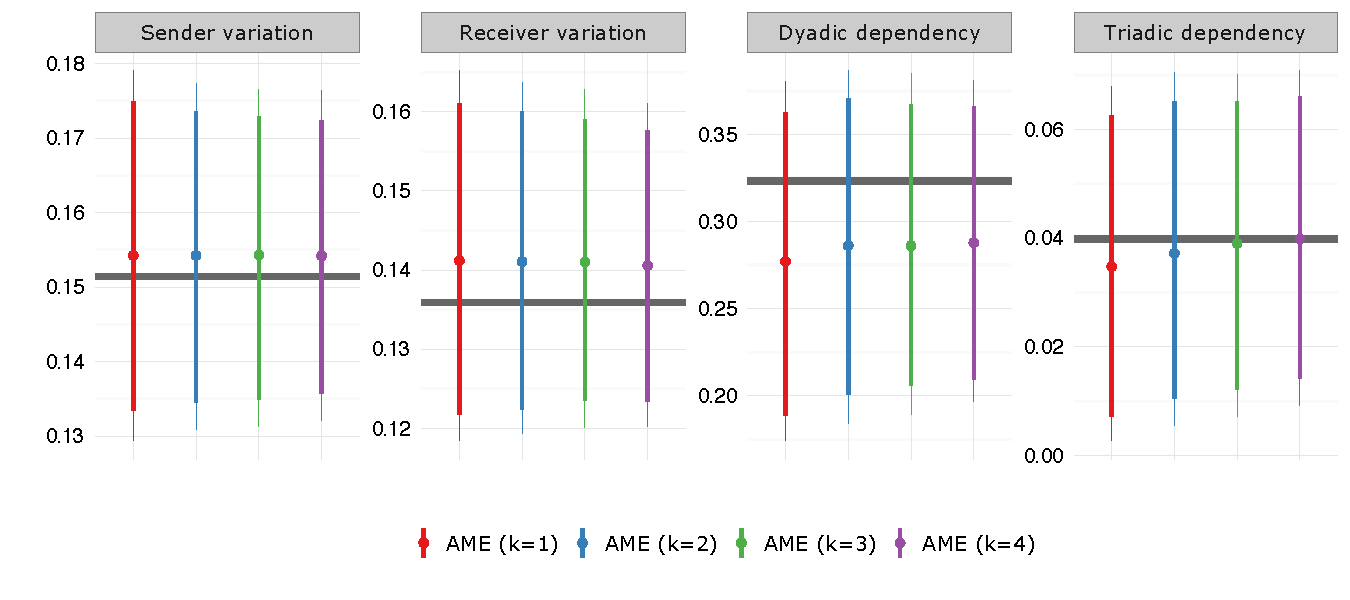
\includegraphics[width=1\textwidth]{netPerfCoef_ameSR}
	\caption{Network goodness of fit summary using \pkg{amen}.}
	\label{fig:netPerfCoef_ameSR}
\end{figure}

% Bib stuff
\clearpage
% \bibliography{/Users/mdw/git/whistle/master}
\bibliography{/Users/s7m/whistle/master}
\bibliographystyle{elsarticle-harv}\biboptions{authoryear}
\newpage

\end{document} 